% !TEX root = /home/frank/School/thesis_text/thesis.tex
% $Id: $


\documentclass[a4paper,12pt]{report}

% The following makes latex use nicer postscript fonts.
\usepackage{times}
\usepackage[dutch,english]{babel}
\usepackage[colorlinks,urlcolor=blue,linkcolor=blue]{hyperref}


 
%%%%%%%%%%%%%%%%%%%%%
%					%
%	VUB Title Page	%
%					%
%%%%%%%%%%%%%%%%%%%%%

\usepackage{vubtitlepage}

\author{			Frank Vanbever}
\title{			Performance Analysis of a Real-Time Video Processing System}

\promotortitle{	Promotors}
\promotor{		Dr. Ir. Erik D'Hollander\\
				Dr. An Braeken}

\advisortitle{	Advisors}					
\advisors{		In. Bruno Tiago Da Silva Gomes}

\faculty{		Faculty of Applied Sciences and Engineering}

\department{		INDI Department}
\reason{			Graduation thesis submitted in partial fulfillment of the requirements
				for\\ the degree of Master of Science in Applied Engineering: Electronics-ICT}
\date{			January 2014}







%%%%%%%%%%%%%%%%%%%%%%%%%%%%%%%%%
%								%
%	Personal Package Includes	%
%								%
%%%%%%%%%%%%%%%%%%%%%%%%%%%%%%%%%


\usepackage{graphicx}
\usepackage{listings}
\usepackage[usenames,dvipsnames]{xcolor}
\usepackage{lscape}
\usepackage{amsmath}
\usepackage{tabularx}
\usepackage{multicol}
\usepackage{float}
\usepackage{booktabs}

%%%%%%%%%%%%%%%%%%%%%%%%%
%						%
%	Personal Settings	%
%						%
%%%%%%%%%%%%%%%%%%%%%%%%%

% set the lenght of the indentation of a new paragraph to 0
\setlength{\parindent}{0pt}

% set some parameters for the listing.
\lstset{language=C,
		belowskip=1em,
		aboveskip=1em,
		basicstyle=\scriptsize,
		keywordstyle=\color{blue},
        stringstyle=\color{red},
        commentstyle=\color{NavyBlue},
        morecomment=[l][\color{magenta}]{\#}
        }


%%%%%%%%%%%%%%%%%%%%%%%%%
%						%
%	Personal Commands	%
%						%
%%%%%%%%%%%%%%%%%%%%%%%%%


\newcommand{\skipbig}[1]{\bigskip #1 \bigskip}
\newcommand{\hlsdirective}[1]{\begin{small} \texttt{#1} \end{small}}

\newcommand{\quotationmarks}[1]{ ``#1''}


%%%%%%%%%%%%%%%%%%%%%%%%%%%%%
%							%
%	DOCUMENT BEGINS HERE	%
%							%
%%%%%%%%%%%%%%%%%%%%%%%%%%%%%

\begin{document}


\maketitlepage

\newpage
\mbox{}

\maketitlepage


% !TEX root = /home/frank/School/thesis_text/thesis.tex


\chapter*{Abstract}

There are many applications that could benefit form increased computing performance. In the past this need was mostly satisfied by Moore's law, which enabled hardware designers and programmers to continue supporting a sequential programming paradigm. However due to power constraints it proved unmaintainable to continue increasing the frequency. The need for processing power however kept rising, and Moore's law is still valid, so parallelism was introduced to enable an increase in performance. The CPU's used in desktop and server computers have become multi-core processors, and alternatives such as General Purpose Graphics Processing Units and Field Programmable Gate Arrays can offer extreme parallelism for applications that can benefit from it. The goal of this thesis is to study a new type of heterogeneous architecture, the Zynq SoC form Xilinx. This chip is a combination of a dual core ARM processor and an FPGA on the same die. Ideally this brings the best features of both processors to the table: the ease of use and floating point performance of the CPU and the massively parallel performance of the FPGA. In the first chapter an introduction is given to the current state of parallel computing. A summary is given of the different types of computing components is given, as well as an introduction to a system for determining which processing unit is most fit to run a certain algorithm. The second chapter gives an overview of the features of the Zynq platform, discussing both the processing system, the programmable logic and the interconnection between these two. The toolchain used to develop for this platform is introduced, as well as the video processing system used to perform the performance analysis. This system, the Zynq Base Targeted Reference Design is a real-time video processing system which has stringent throughput requirements. The complete stack is discussed: the hardware implementation, the operating system and the user application. In the third chapter details High Level Synthesis, a technique for converting high level programming languages into hardware. The many features of the tool used for this thesis, Vivado HLS, are also discussed in this chapter. In the fourth chapter the factors influencing the performance are discussed, as well as the roofline model, a way to visually represent the performance of a system. Concepts form this roofline model are used to interpret the performance of the system.
% !TEX root = /home/frank/School/thesis_text/thesis.tex

\chapter*{Abstract (NL)}

\begin{otherlanguage}{dutch}


Er zijn vele toepassingen die baat hebben die baat hebben bij een toegenomen performantie van de computer die ze uitvoert. In het verleden zorgde “Moore's Law” ervoor dat ontwerpers en programmeurs het sequentiële paradigma konden blijven toepassen. Door limieten in de fysica van halfgeleiders werd het halverwege het vorige decennium onhoudbaar om dit model te blijven volgen. De nood aan extra performantie bleef echter bestaan, en Moore's law was nog steeds gelding. Omwille van deze redenen werd parallellisme geïntroduceerd om voor bepaalde parallelle toepassingen te gaan versnellen. Vandaag hebben processoren in desktops en servers een multi-core processor aan boord, en alternatieven zoals de GPGPU of de FPGA kunnen extreem parallellisme bieden voor applicaties die hier baat van kunnen hebben.
Het doel van deze thesis is om de performantie van een nieuw type heterogene architectuur te bestuderen, de Zynq SoC van Xilinx. Deze chip combineert een dual core ARM processor en een FPGA op dezelfde chip. Idealiter zou deze de voordelen van deze beide moeten samenbrengen in 1 verpakking: het gebruiksgemak en performantie bij floating point berekeningen van de CPU en het doorgedreven parallellisme van de FPGA.
In het eerste hoofdstuk wordt een introductie gegeven tot de huidige toestand van parallel processing. De meest courante parallale processors worden beschreven evenals een systeem voor het classificeren van parallelle algoritmes. Het tweede hoofdstuk begint met een beschrijving van het Zynq platform, waarbij de processor, de FPGA als de verbindingen tussen deze 2 besproken worden. Het video bewerkings-systeem dat gebruikt wordt voor deze thesis, de Zynq Targeted Reference Design is een real-time video bewerkings-systeem met strenge vereisten voor de doorvoer van het systeem. De volledige stack wordt besproke, gaande van de hardware over het besturingssysteem tot de eigenlijke applicatie. In het derde hoofdstuk wordt uitgelegd wat High Level Synthesis is, een techniek om een programmeertaal om te zetten naar hardware. De eigenschappen van Vivado HLS, de gebruikte software, worden ook in dit hoofdstuk besproken. In het vierde hoofdstuk worden de factoren die de performantie van het systeem beïnvloeden besproken, evenals een systeem om de performantie visueel weer te geven:  het roofline model. Concepten van dit roofline model worden gebruikt om de performantie te interpreteren. 

\end{otherlanguage}
% !TEX root = /home/frank/School/thesis_text/thesis.tex


\chapter*{Preface}

% Obligatory lists
\tableofcontents
\listoffigures
\listoftables

% !TEX root = /home/frank/School/thesis_text/thesis.tex




\chapter{Introduction} 
Up until halfway the first decade of the new millennium it was possible to gain computing performance whilst also being able to maintain the sequential programming paradigm. This was due to Moore's law, stating that the number of transistors on integrated circuits double approximately every two years. There was no need for research into explicit parallelism because the next generation of computing devices was just around the corner which would make the research obsolete.To perpetuate the sequential programming paradigm several innovations such as multiple issue, deep pipelines and out of order execution were introduced into processors which were inefficient in both the use of transistors and power.  Eventually though it became impossible to progress any further whilst still supporting the sequential paradigm. The integrated circuit industry was unable to continue decreasing the size of MOSFETs whilst continuing to increase the clock frequency. The industry had hit what is called the power wall.
The solution to this problem was to go over to parallel processors, meaning that there is more than one processing unit working at a time. A lot of real world applications are parallel, and hardware can be made parallel with relative ease. The problem lies in the programming model, how to exploit this parallelism and make programming for these parallel architectures easier and transparent for the programmer.

\section{Computing Components}

\subsection{Multicore Processor}
The multicore processor is the solution presented for the aforementioned problems by the traditional CPU manufacturers such as Intel and AMD. The idea behind this type of processor is to place a number of cores (currently up to eight) on the same die. This presents a compromise between maintaining sequential performance whilst also providing a certain advantage of parallel processing. Parallel programming for these processors presents certain challenges whilst their modest parallelism cannot provide a dramatic improvement in power performance. Multicore processors are unlikely to be a one-size-fits-all solution to the parallel problem.\cite{asanovic_landscape_????}

\subsection{Graphics Processing Units} Graphics Processing Units
Graphics processing units are a type of coprocessor in in traditional computers meant to process images for output to the display. Recently however there has been increased interest in the GPGPU, the general purpose graphics processing unit. These processors implement a different paradigm, namely the manycore paradigm. A  GPU is a processor with hundreds single instruction multiple data cores, each of which is heavily multi-threaded. Because of this large amount of cores the FLOPS (floating point operations per second) is unrivaled\cite{kirk_programming_2010}. GPU's, due to their SIMD nature present some problems, conditional execution paths for example, present a serious overhead on the GPU. GPU's are programmed with either OpenCL (open standard) or CUDA (proprietary to Nvidia)

\subsection{Field Programmable Gate Array} 
FPGAs are devices containing a vast amount of configurable logic linked by programmable connections. This logic is comprised of lookup tables grouped together into configurable logic blocks. Any combinatorial function can be programmed into these LUT's. Next to these uncommitted logic blocks a typical FPGA also contains several blocks with a specific function such as block ram and DSP multipliers. FPGAs are an interesting competitor in the parallel processing field because they aren't constrained by the Von Neuman architecture. FPGAs follow the dataflow paradigm in which the data “flows through the logic. Implementing a data-flow is inherently parallel. The different stages in the datapath can also be made sequential effectively making the datapath a pipeline. The fine grained nature of FPGAs also means that the bitwidth can be adapted to the application.


\section{Berkeley Dwarves}

Image processing algorithms are very compute intensive. These makes them prime targets for exploiting parallelism and implementing them on parallel architectures. Which platform is the best fit however is dependent on both the algorithm and the data. A common method to subdivide parallel algorithms is presented in , the so called \emph{dwarfs}. These 13 dwarves are classes of algorithms in which the membership is defined by a similarity in computation and data movement.These 13 dwarfs are classes of algorithms in which the membership is defined by a similarity in computation and data movement.
The dwarfs are:

\begin{multicols}{2}
\begin{enumerate}
\item Dense Linear Algebra
\item Sparse Linear Algebra
\item Spectral Methods
\item N-Body Methods
\item Structured Grids
\item Unstructured Grids
\item MapReduce
\item Combinational Logic
\item Graph Traversal
\item Dynamic Programming
\item Backtrack and Branch-and-Bound
\item Graphical Models
\item Finite State Machines
\end{enumerate}
\end{multicols}

A thorough review of these dwarfs and what kind of computation and communication they entail goes beyond the scope of this document. More information can be found on the Berkeley View Wiki \cite{anon._dwarf_????} and an updated view can be found in \cite{asanovic_view_2009}.\\
Finding out which dwarf is most suited for which platform is a very labour-intensive task. In \cite{inta_chimera:_2012} a theoretical analysis of dwarf performance on different accelerators in heterogeneous systems is given. A first point to note is that for floating point operations GPU's are hard to beat. Fixed point numbers are a way to overcome this problem. Another point to note is that conditional elements and  costly communication can wreak havoc on the accelerator's performance. In Figure \ref{img:venndiagram_chimera} the analysis is represented by a Venn diagram. In this diagram * denotes fixed point operations whilst \^{} denotes floating point operations.

\begin{figure}[H]
\centering
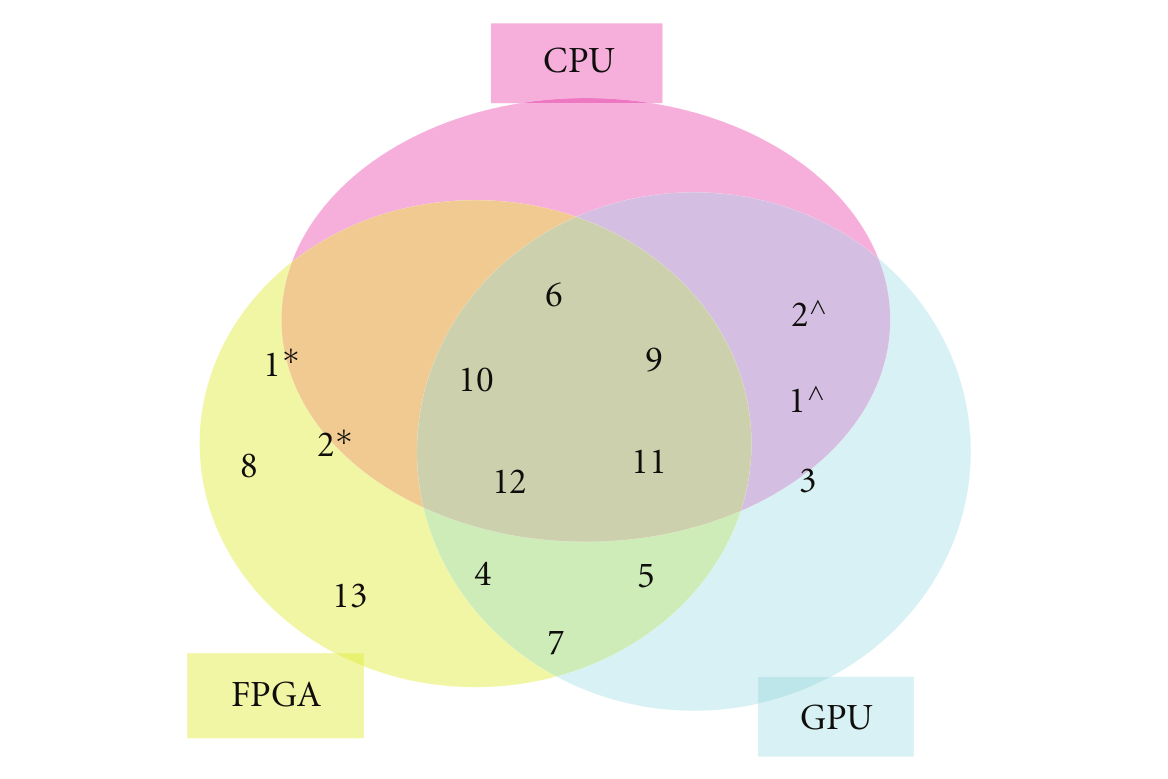
\includegraphics[scale=0.34]{/home/frank/School/thesis_text/images/venndiagram_chimera.png}
\caption{Analysis of different hardware accelerators in regards to performance on a certain dwarf \cite{inta_chimera:_2012} }
\label{img:venndiagram_chimera}
\end{figure}


\section{GUDI Project}

This thesis is inspired by the work of the GUDI project. GUDI is an acronym for \quotationmarks{A Combined \textbf{G}P-GP\textbf{U}/FPGA \textbf{D}esktop for accelerating \textbf{I}mage processing applications}. The research starts from the observation that there is a large need for computing power to process data using computationally intensive image processing algorithms. Conventional Off-the-shelf Desktop computers don't have the necessary processing power to satisfy this demand. A lot of image processing algorithms exhibit parallelism which can be exploited by the right architecture. Two such massively-parallel architectures are GP-GPU's and FPGA's. The GUDI project has for goal to investigate the possibilities and limitations of a computer with such a heterogeneous architecture. It is an investigation into which technologies and which development tools perform best in different situations. The means through which this is done is through the implementation and performance measurement of algorithms. The ultimate goal is to split an algorithm into several parts which are executed on the technology (CPU,GPU,FPGA) most fit for the job so as to ensure optimal speed-ups.





% !TEX root = /home/frank/School/thesis_text/thesis.tex



\chapter{Platform Overview}

\section{Zynq-7000}

The Zynq-7000 System on Chip combines a dual core ARM Cortex-A9 with Xilinx programmable logic in a single device. This combination of a CPU and an FPGA on the same device is not a new phenomenon, with examples of previous generations being the PowerPC based Xilinx Virtex-II Pro and some models of the Virtex 4 and Virtex 5 series FPGA's. The two most notable differences between these generations is the shift from PowerPC based architectures to ARM based architectures, and a notable shift in emphasis from HDL centered design to a more programmer centric view with an emphasis on high level languages. 
	

	\subsection{Processing System}
	The Zynq-7000 series SoC is split into two parts: The processing system (PS) and the programmable logic (PL). The Processing system (PS) contains an Application Processor Unit (APU), memory interfaces and I/O peripherals. 
	
		\paragraph{APU}
		The APU is a Dual ARM Cortex-A9 CPU which implements version 7 of the ARM ISA  as well as Thumb and Jazelle instruction sets. Each core has a NEON Media Processing Engine supporting SIMD vector and scalar single-precision floating-point and integer computation and scalar double-precision floating-point computation. Each core has 32 KB instruction and 32 KB data caches and there is 512 KB shared L2 cache and 256 KB of on-chip SRAM memory. The APU also has a snoop control unit to maintain L1 and L2 coherency. This snoop control unit also controls the Accelerator Coherency Port, a 64-bit AXI slave port from the programmable logic, which performs the role of master, to the processing system which serves as slave. This allows direct communication between the PS and the PL through the L2 caches or on chip memory with guaranteed coherency. The also has an on-board 8-channel DMA controller with 4-channels reserved for PS to/from memory and 4 for PL to/from memory transfers. Finally the Processing system also contains an interrupt controller.

		\paragraph{Memory Controller}
		The Memory controller supports a number of memory technologies. The system has a DDR controller which supports DDR2 and DDR3 memory, a Quad-SPI controller which converts normal memory read operations to SPI and vice versa, and a Static Memory Controller which supports NAND and SRAM/NOR type memory.

		\paragraph{I/O Peripherals}
		The Processing system contains quite a lot of industry standard I/O peripherals for external data communication.
			\begin{multicols}{2}
				\begin{itemize}
					\item GPIO
					\item 2 Gigabit Ethernet Controllers
					\item 2 USB controllers
					\item 2 SD/SDIO controllers
					\item 2 SPI controllers
					\item 2 CAN controllers
					\item 2 UART controllers
					\item 2 I$^{2}$C controllers
				\end{itemize}
			\end{multicols}

		These peripherals are connected to multiplexed I/O buffers which enable to externalize these signals to up to 54 pins. If there is a need for more I/O pins the signals can be routed into the PL through the extended MIO, where they can be routed directly to package pins or peripherals in the PL.

	\subsection{Programmable Logic}
	The programmable logic provides the same functionality that can be expected from a Xilinx FPGA. The PL in 7z010 and 7z020 Zynq SoCs is based on Artix-7 FPGAs whereas the PL in 7z030, 7z045 and 7z100 SoCs is based on Kintex-7 FPGA logic. This PL can be coupled through a couple of different interconnects, with varying degrees of interconnectedness between the PL and the PS. Of note here is that the PS has to be booted first and the PL logic has to be configured from the PL at boot or at a later time. This is another example of the shift to a more software centered view. The system has all the features one can expect from an FPGA: configurable logic blocks with look-up tables, a number of 36 KB block RAMs, DSP348E slices and configurable IO. The PL side also contains an Analog to Digital converter, and in the larger varieties of the Zynq SoC an integrated PCI Express block.

\begin{figure}[H]
\centering
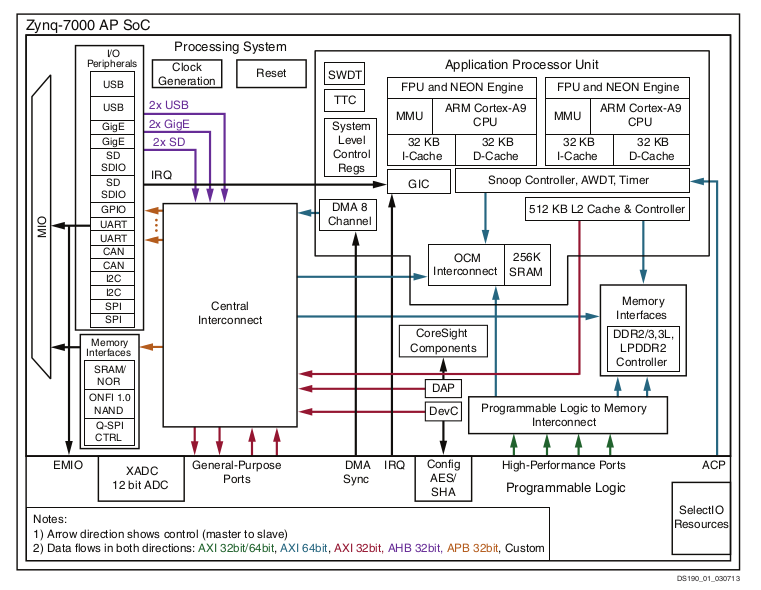
\includegraphics[scale=0.5]{/home/frank/School/thesis_text/images/zynq_block_diagram.png}
\caption{Zynq -7000 SoC overview \cite{anon._zynq-7000_2013}}
\label{img:zynq_overview}
\end{figure}

	\subsection{Interconnect}
	The interconnect system is located in the PS but because of it's influence on performance it warrants its own section. The interconnect system is comprised of a number of switches to connect the different parts of the system using the AXI point-to-point protocol. The AXI protocol is part of the ARM Advanced Microcontroller Bus Architecture version 3.0. These AXI interconnects are the primary means of communication between the PS and the PL. There are a number of different interface ports between the PS and the PL:

		\begin{description}
			\item[AXI\_HP] There are four AXI\_HP interfaces, connecting PL masters with high bandwidth datapaths to the DDR and OCM memories. Each interface is buffered with 2 FIFOs and is configurable to be 32 or 64 bits wide.
			\item[AXI\_GP] The four general purpose AXI\_GP ports are divided into 2 master ports and 2 slave ports. These ports don't have FIFO buffering which makes them less suitable for high performance use. 
			\item[AXI\_ACP] The Accelerator coherency port is a 64-bit AXI slave interface that directly connects the PL to the APU caches. This is done through the snoop control unit and can enforce coherency if requested. 
		\end{description}

	The actual interconnection is done through a number of switches. Amongst these are the snoop control unit, the L2 cache controller and a couple of ARM NIC-301 based interconnect switches.

		\begin{description}
			\item[Snoop Control Unit] Although the SCU is in essence not a switch, its behavior in regards to the transfer of data from its AXI slave ports to its AXI master ports makes it function as a switch.
			\item[Central Interconnect] The central interconnect is the core of the interconnect network in the Zynq SoC.\
			\item[Master Interconnect] The master interconnect connects the Master switches the traffic from the AXI\_GP ports as well as traffic coming from the device configuration core and the debug access port.
			\item[Slave Interconnect] The slave interconnect switches traffic comming from the central interconnect to AXI\_GP, I/O peripherals, APB connections, etc.
			\item[Memory Interconnect] The memory interconnect switches high speed traffic comming from the AXI\_HP ports to DDR and on-chip RAM.
			\item[OCM Interconnect] The on-chip memory connect switches the traffic from the central interconnect and the memory interconnect.
		\end{description}

		A diagram of the way these interconnects are organized can be found in figure \ref{img:zynq_intereconnect}

\begin{figure}[H]
\centering
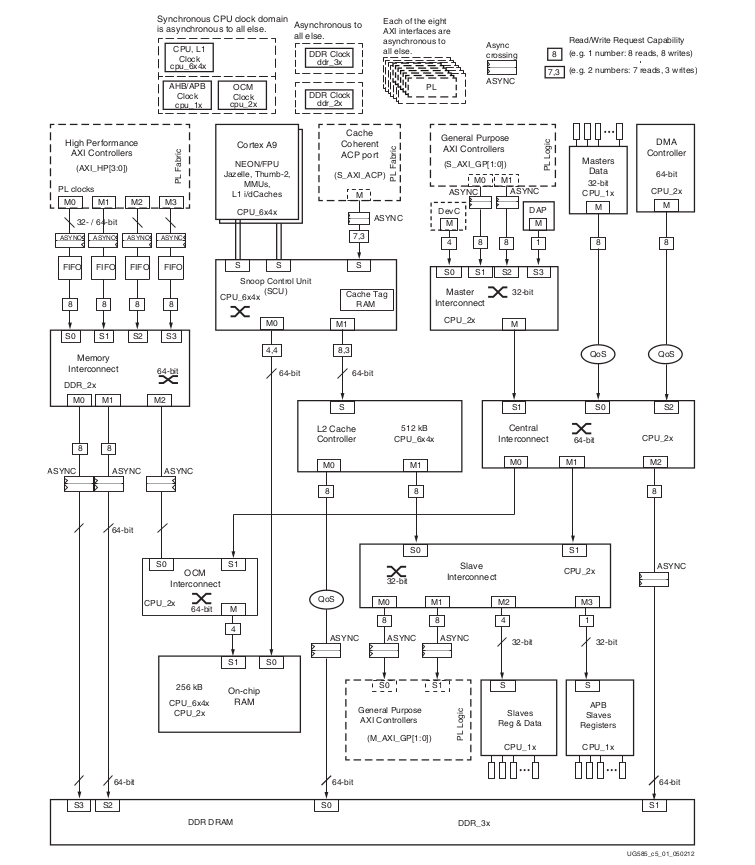
\includegraphics[scale=0.55]{./images/interconnect_block_diagram.png}
\caption{Zynq Interconnect System Block Diagram \cite{anon._zynq-7000_2013}}
\label{img:zynq_intereconnect}
\end{figure}

\section{Toolchain}
Because of the heterogeneous nature of the Zynq Soc there are a number of tools necessary to implement a design. In this section the tools used for this thesis are discussed.

\paragraph{PlanAhead} PlanAhead is the main interface for the hardware side of a project. It allows a designer to bring together VHDL or Verilog code, IP-cores, embedded designs from Xilinx Platform studio and DSP designs from System generator. It also integrates with ISE Simulator to allow the functional verification of HDL code and IP. PlanAhead also allows the insertion of Chipscope cores to debug RTL designs.

\paragraph{Xilinx Platform Studio (XPS)} Xilinx platform studio is a graphical tool that allows a designer to build embedded processor systems including IP-cores. Connecting peripherals in the PL to the PS of the Zynq is done through this application.

\paragraph{Vivado HLS} Vivado HLS is a high-level synthesis tool that converts C, C++ and SystemC to synthesizable hardware. It can export this hardware into a number of formats, among which the PCore format for XPS. More on Vivado HLS can be found in section \ref{sec:vivado_HLS}

\paragraph{Xilinx SDK} Xilinx' Software Development Kit is an eclipse based integrated development environment targeting the ARM core in Zynq or the Microblaze softcore processor. It includes a complete GNU based compiler toolchain in the form of the Mentor Sourcery Codebench Lite - Xilinx edition, zhich also incorporates debugging and profiling tools. The SDK also has plugins which make it aware of the peripherals placed in the PL. The SDK also has a library of drivers for Xilinx IP-cores.

The necessary steps for developing a design for the Zynq SoC are as follows:

\begin{enumerate}
	\item Start the project in PlanAhead, specify the parameters of the hardware you're developing for and create a new embedded design
	\item Independent of the PlanAhead project, implement the algorithm using Vivado HLS so it statisfies all design constraints. Export the implementation as an IP-core suitable for use in XPS.
	\item In XPS, add the Vivado HLS generated IP core to the system along with other IP-cores necessary for the functioning of the system. Make all the necessary interconnections.
	\item Add the necessary floor-planning constraints in PlanAhead. Synthesize the system, perform the implementation step on the system and generate a bitstream. Correct any errors that show up during these steps until the system is error-free.
	\item Export the system to SDK. In SDK, develop the embedded software using the available drivers. Create a boot image combining the software and the hardware and launch the application on the hardware.
\end{enumerate}
These steps are visually represented in figure \ref{img:toolchain_diagram}

\begin{figure}[H]
\centering
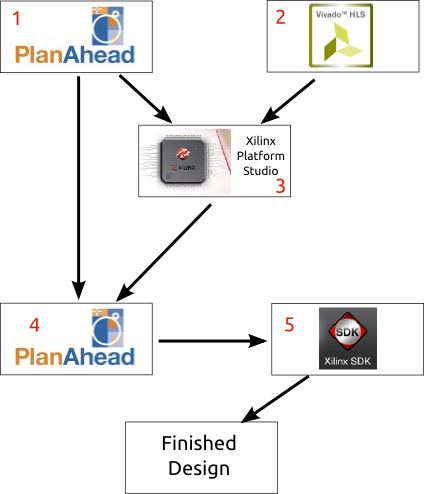
\includegraphics[scale=0.7]{./images/toolchain_diagram/toolchain_diagram.png}
\caption{Diagram of the Zynq toolchain}
\label{img:toolchain_diagram}
\end{figure}

Xilinx provides an alternative toolchain in its Vivado Design Suite. It supports the Zynq-7000 series since the release of version 2013.3 in October 2013. This software combines the functions of PlanAhead and XPS into one application.For new designs using 7-series and Zynq devices Xilinx recommends using Vivado Toolchain, With the old ISE toolchain still being available for backward compatibility reasons.\cite{isereleasenotes}.
 Xilinx


\section{Base Targeted Reference Design 14.5}
Zynq is a powerful but complex architecture requiring that a designer has different skills. Building a real-time video processing from scratch would involve connecting multiple IP-cores to each other and to the PL, as well as writing efficient applications that use the implemented hardware. Because this falls beyond the scope of this thesis an existing design was selected to do a performance analysis on. The Base Targeted reference Design version 14.5 was chosen because it utilized a Vivado HLS accelerator as well as some features of the Zynq architecture promising high performance and it was especially developed for the available hardware. 

\subsection{Hardware}
The hardware side can be split into 3 stages. The first stage starts with the \emph{fmc\_imageon\_hdmi\_in} IP-core. This core extracts the horizontal and vertical blanking signals from the YCrCb 4:2:2 input it receives from the FMC-Imageon Module. This core is connected to the \emph{Video In to AXI4-Stream} IP-core. This core handles the clock boundary between the video clokc domain and the AXI4-Stream clock domain. The preservation of timing information is guaranteed by a Video Timing Core. The AXI4-stream is routed into a \emph{Test Pattern Generator} IP-core which can generate a test-pattern or act as a pass-through for the video signal, depending on the configuration. The data coming from the TPG is fed into a \emph{Chroma Resampler} IP-core which converts the YCrCb 4:2:2 formatted signal into a YCrCb 4:4:4 signal. HDMI uses the chroma subsampling to reduce the amount of data that needs to be transmitted. This can be done because the human eye is not as sensitive for the Chroma components as it is for the Luminance component. The upsampling is necessary for the following step, which is the colorspace conversion performed by the \emph{YCrCb to RGB Color-Space Converter} IP-core. This core converts the YCrCb signal to RGB video as this is the format required by the following steps in the video processing pipeline. The video signal gets routed into a \emph{Video DMA}controller which writes the data to memory using an \emph{AXI Interconnect} IP-core connected to the PS' S\_AXI\_HP0 port.\\
The second stage has a second \emph{AXI Interconnect} IP-core connected to the PS' S\_AXI\_HP2 port. A \emph{Video DMA} controller reads data from memory through this interconnect and converts the AXI form the memory mapped format to an AXI stream format. This gets sent to the Vivado HLS generated Sobel core. This core sends the data back to the Video DMA controller which writes it back to memory through the AXI Interconnect.
The Third and last stage consists of the Xylon logiCVC-ML which is connected to the first AXI Interconnect. This is a video display controller which reads the data from the video memory and converts it into a format suitable for output. It also generates the control signals for the output.\\
The IP-cores that use AXI-Lite for their configuration are also connected to a third AXI Interconnect IP-core. This IP-core is connected to the M\_AXI\_GP0. Through this connection is the PS able to control the functioning of the video processing pipeline. Finally There is an AXI Performance Monitor IP-core also connected to this third interconnect. The Performance monitor monitors the througput on the S\_AXI\_HP0 and S\_AXI\_HP2 ports. 





\subsection{Software}
On the software side the TRD uses three major components:
\begin{itemize}
	\item Boot Loader
	\item Xilinx Linux Kernel
	\item Application
\end{itemize}

\subsubsection{Boot Loader} The TRD uses the SD card to boot form. The boot loader is stored in the BOOT.BIN file and performs a number of functions. The system uses a two-stage boot loader. On boot the first stage boot loader gets executed, which performs the necessary initializations that enable the system to load the bitstream into the PL and execute the U-Boot bootloader. The bitstream is also contained in the BOOT.BIN file and is loaded into the PL after the initialisation is done. After the FSBL has finished it executes the second stage, the U-Boot boot loader which loads the kernel image into the DDR memory.

\subsubsection{Linux Kernel}
The TRD uses a Linux kernel that is based on the mainline Linux kernel but maintained by Xilinx. This kernel incorporates many patches not found in the mainline kernel that provide drivers for many Xilinx IP-cores. Supported devices include the Xylon logiCVC-ML which gets abstracted to a generic frame buffer drive, Xilinx VDMA controllers which controls the transfers to and from the DDR memory, PS-GPIO giving access to GPIO pins to the operating system, and the ADV7511 HDMI transmitter gets a Video4Linux v2 Driver. Some IP cores have limited functionality and don't warrant a complete Kernel Driver being written to support the driver. In this case the developer can use the \emph{Userspace IO} framework present in the Linux kernel.\\
Userspace IO or UIO is a framework present in the Linux kernel that allows a developer to write a minimal kernel driver for a piece of hardware and perform most of the necessary functions from userspace. This system reduces the complexity of driver development and reduces the risk for bugs in a kernel module. UIO is a good fit for a device if it has one or more of following properties:
\begin{itemize}
	\item The device has memory that can be mapped onto virtual memory and can be completely controlled using this memory.
	\item The device generates interrupts
	\item The device doesn't fit in one of the standard kernel subsystems.
\end{itemize}

These UIO device drivers are made available to the user through the device node and the Sysfs, which is a virtual file system that exports information on devices and their drivers. The device file typically has the form /dev/UIOX with X being a number starting on 0. This file represents the memory of the system and can be opened using the MMAP() system call. Interrupts are handled by performing a blocking read on the device file. When the read returns an interrupt has happened. This read returns an integer which contains the number of interrupts that have occurred. By comparing this value to the previous value the user can check whether any interrupts were missed. Vivado HLS generates the UIO driver, leaving only the development of a kernel module to be done by the developer.

\subsubsection{Application}
There are 2 versions of the application available: a version with a Qt based GUI and a commandline based application. The application lets the user to select between 2 video sources, the TPG or the HDMI input, and apply 2 implementations of the Sobel filter on these inputs. One implementation is done in software and runs on ARM processor, the other one is a vivado HLS generated core. The Qt application also has a readout of the throughput of the system.


\subsection{Sobel Operator}

The described system performsedge detection using the sobel operator on the video data. The sobel operator computes an approximation of the gradient. The computation is done by convolving the image with 2 $3 \times 3$ kernels.

\begin{equation}
G_{x} = 
\begin{bmatrix}
+1 & 0 & -1 \\
+2 & 0 & -2 \\
+1 & 0 & -1
\end{bmatrix}
\hspace{20mm}
G_{y} = 
\begin{bmatrix}
+1 & +2 & +1 \\
0 & 0 & 0 \\
-1 & -2 & -1 \\
\end{bmatrix}
\end{equation}

The combination of these operators give an approximation of the gradient in both the x and the y direction. The sum of the absolute values of these two approximations gives the edge weight. It shows whether a location is close to an abrupt change in intensity in an image, an edge. By thresholding the edges can be separated from the rest of the image. The Sobel operator falls under dwarf number 6: structured grid which puts it in the cross section of the CPU, GPGPU and FPGA categories. The sobel oparator is thus a good fit for the Zynq platform. 
% !TEX root = /home/frank/School/thesis_text/thesis.tex


\chapter{High Level Synthesis}



A recurring theme in the literature is the relative difficulty of implementing an algorithm on an FPGA compared to conventional implementation techniques on CPU's and GPU's. Both development time and place-and-route take considerably more time compared to programming/compiling for more traditional architectures \cite{inta_chimera:_2012,tsoi_axel:_2010}. With an increase in the complexity required to perform a task also comes an increase in the difficulty of designing and debugging such a system. 
High level synthesis tools enable a user to specify the behavior of a system in a high level programming language and convert this description into usable hardware. Most tools use the C, C++ or sytstemC programming languages, however other programming languages such as the functional programming language Haskell \cite{baaij2010c}, the scripting language Pythonh\cite{decaluwe2004myhdl} or Matlab M-code\cite{hdlcoder} have been used. These tools enable faster prototyping and implementation\cite{che_accelerating_2008}. These tools also enable programmers without a background in HDL design to benefit from the advantages of FPGA accelerators without facing the steep learning curve of learning a HDL such as VHDL or Verilog. For existing HDL designers HLS tools these tools present a reduction in the number of lines of code that are needed to describe the design\cite{casseau_c-_2005}. 
These tools enable to shift the focus from low-level implementation details to the development and improvement of the algorithm in a rapid prototyping fashion\cite{wakabayashi_c-based_2004}.
HLS tools have a long history dating back to the 1970's but only recently have these tools matured enough to become adopted by industry. These tools present an interesting evolution and a possible paradigm shift in hardware design and prototyping\cite{cong_high-level_2011}.



\section{Riverside Optimising Compiler for Configurable Computing} 
ROCCC is a C-to-vhdl compiler which focusses on FPGA based code acceleration. It implements a subset of the C language on which it performs loop analysis techniques to provide increasing throughput with less usage of area\cite{martin_high-level_2009}. The generated VHDL is independent from FPGA platforms and supports code reuse through the use of modules. 
ROCCC uses the streaming paradigm, in which data is represented by streams, a data format similar to the way arrays are stored in memory. These streams pass through a set of operations called kernels. This way of representing data makes it possible to express parallelism and is relatively easy mapped to the FPGA hardware. This paradigm removes the need for area-costly soft-core processors\cite{buyukkurt_impact_2006}.\\
This streaming paradigm is also what enables the platform independence of the ROCCC hardware. As long as the data is delivered to the system in the form of a stream it can be used.
Another important feature of ROCCC are the so-called smart buffers. These attempt to utilize the data-locality of certain applications to increase the performance. This is done by utilizing intelligent data reuse to minimize the number of off-chip memory acceses. 

\section{Xilinx Vivado High Level Synthesis Tool}
\label{sec:vivado_HLS}
Vivado High-Level Synthesis is part of the Xilinx Vivado design suite and is the product of the acquisition of AutoESL and the re-branding of their AutoPilot High-Level Synthesis tool. Vivado represents the next evolution of Xilinx tools fitting in their vision of an \quotationmarks{all programmable world}.  It allows C, C++ and SystemC code to be synthesized into VHDL or Verilog code. Functional simulation can be done in C, which is a great improvement over the typical VHDL or Verilog simulation. The Vivado tool is based on the Eclipse platform and incorporates the C Development tool (CDT).[15]
\\
Vivado HLS was as the HLS tool for this thesis because of it's integration in the Xilinx Toolchain and \emph{out-of-the-box} support for the Zynq platform.

\subsection{
}

% !TEX root = /home/frank/School/thesis_text/thesis.tex

\chapter{Performance Analysis}

\section{Pragma's influencing the memory architecture implementation}

The way memory accesses are implemented are an important factor influencing the performance of an IP-Core. Buffers have a large influence on the operational intensity. Increasing operational intensity moves the implementation from memory bound area of the roofline model to the compute bound area of the roofline model.\\
In \emph{High Level} programming languages memory gets abstracted to variables and array's. These abstractions need to be translated into something that can be implemented in hardware. For FPGA's this means choosing between \emph{block ram} or registers. The process of translating the memory constructs into the most fitting type of physical memory is controlled by the HLS compiler but can be influenced by using directives or pragma's. Especially the way arrays are translated into hardware is of importance. For this purpose a couple of directives are available.\\

\begin{description}

\item[Resource] lets the programmer determine which component will be used to map a certain array to.

\item[Array\_Map] Maps several smaller arrays to the same memory to decrease the resource consumption.

\item[Array\_Partition] Determines how a certain array will be partitioned into smaller arrays each using their own memory to avoid the bottleneck of having to perform multiple consecutive reads. This directive also allows to partition an array completely into registers.

\item[Array\_Reshape] Will rearrange an array so the elements have a larger word width. This improves the performance of the memory while maintaining the same resource consumption.

\end{description}

In systems doing video processing buffers are usually employed to exploit the spatial and temporal data locality. In the example of the TRD there are 2 abstractions implemented: \texttt{ap\_linebuffer} and \texttt{ap\_window}.

\subsection{\texttt{ap\_linebuffer} Class}

The class \texttt{ap\_linebuffer} is a generic C++ implementation of the linebuffer described in XAPP793. A linebuffer is described as a multi-dimensional shift-register. A linebuffer needs to be able to be read and written to in the same cycle to maximize performance. The dual port nature of block RAM makes it the ideal component for this abstraction.
Because the \texttt{ap\_linebuffer} class is generic its behavior needs to be defined in the application. The template for the \texttt{ap\_linebuffer} class is \texttt{<typename T, int LROW, int LCOL>}. A type, the number of rows and the number of columns need to be specified. This is done in the \texttt{sobel.h} file by the following line:


\skipbig{\hlsdirective{typedef ap\_linebuffer<unsigned char, 3, MAX\_WIDTH> Y\_BUFFER;}}


The parameters of the template are used to determine the size of the only variable of the class, -the array M of type T with LROW rows and LCOL columns.\\
This array get partitioned by the following directive:

\skipbig{\hlsdirective{\#pragma AP ARRAY\_PARTITION variable=M dim=1 complete}}


This means that the first dimension, the number of rows, get partitioned into different block RAMs. This is also reported by the vivado HLS tool. buff\_A is the line buffer used throughout the implementation.\\

\medskip

\begin{figure}[h]
\centering
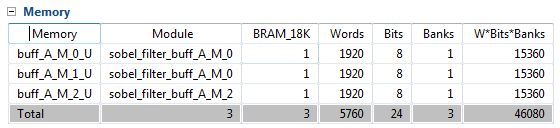
\includegraphics[scale=0.8]{/home/frank/School/thesis_text/images/trd_original_buffer_partitioning.PNG} 
\caption{paritioning of an array in multiple block RAM instances}
\end{figure}


\subsection{\texttt{ap\_window} Class}

The second class used in the application is a generic implementation of the memory window described in XAPP793. It is a combination of shift-registers forming a 2-dimensional data storage element of N pixels centered on a pixel P. Usually these are implemented as flip-flops because they contain relatively few elements who need to be simultaneously available for a calculation. This is achieved through completely partitioning the memory into registers, preventing it from being implemented by a block RAM.
The template of \texttt{ap\_window} is \texttt{<typename T, int LROW, int LCOL>}. These parameters are used for the only variable in the class, an array M of type T with LROW rows and LCOL cols. Analog to the linebuffer class the programmer here also needs to define the type, number of rows and number of columns of array M. The array gets paritioned into registers by the following directive:


\skipbig{\hlsdirective{\#pragma AP ARRAY\_PARTITION variable=M dim=0 complete}}


The \texttt{dim=0} means that all dimensions should be partitioned. The \texttt{complete} keyword signifies that this partitioning should be done for the whole array.


\subsection{influence of memory architecture on the operational intensity}

This hierarchical structure of the memory influences the operational intensity of the algorithm. The numerator is determined by the number of bytes being processed by the core. Every iteration one value gets read from the external memory and one value gets written.  There are 32 bits per pixel, so there are 4 bytes per pixel. this means that with height H and width W there are:

\[
4 * 2 * ( H * W )
\]

bytes being read/written to/from the memory. This is the denominator in the expression of the operational intensity.\\
The numerator is dependent on the number of pixels being calculated by the core. The core used in the TRD doesn't calculate the pixels on the outer rim of the image and instead uses these as padding. 

\begin{lstlisting}

if( row <= 1 || col <= 1 || row > (rows-1) || col > (cols-1)){
		
		edge.R = edge.G = edge.B = 0;
		
}
//Sobel operation on the inner portion of the image
else{

		edge = sobel_operator( ... );
		
}		
\end{lstlisting}

This branching needs to be taken into consideration for the expression of the computational intensity. The expression for the numerator is given by:

\[
( H * W ) -[ ( 4 * W ) + 4 * ( H - 4 )]
\]


the complete expression is then given by:

\[
\frac{( H * W ) -[ ( 4 * W ) + 4 * ( H - 4 )]}{4 * 2 * ( H * W )}
\]








\section{Pramga's influencing throughput}

\subsection{Original TRD}

The original TRD has 3 pragma's applied to it:

\begin{itemize}
\item \hlsdirective{set\_directive\_loop\_flatten -off \\ "sobel\_filter/sobel\_filter\_label0"}
\item \hlsdirective{set\_directive\_dependence -variable \&buff\_A -type inter \\ -dependent false "sobel\_filter/sobel\_filter\_label0"}
\item \hlsdirective{set\_directive\_pipeline -II 1 \\ "sobel\_filter/sobel\_filter\_label0"}
\end{itemize}



These all influence the system in a distinct way.

\paragraph{Loop Flattening} This directive combines nested loops. This removes the need for the clockcycle needed to enter and leave the loop. It needs to be applied to the inner loop of a set of nested loops. In the TRD loop flattening is explicitly disabled.

\paragraph{Dependence} The compiler tries to identify dependencies between calculations or resources. Sometimes this automatic identification of dependencies is too conservative because the compiler doesn't have some information. For this reason the \emph{dependence} directive exists, allowing the programmer to explicitly state that there are or aren't dependencies for a certain variable. There are two types of dependence:

\begin{description}
\item[Inter] The dependence is between different iterations of the same loop. If the dependence is set to false this will allow the loop to be unrolled
\item[Intra] The dependence is inside the iteration. If the dependence is set to be false the compiler will attempt to reorder the operations for the most optimal performance.
\end{description}

In the case of the TRD the inter-dependence of the variable buff\_A is set to false.

\paragraph{Pipeline} The directive set\_directive\_pipeline is used to control the pipelining of loops and functions. Each function or loop on which this directive is used can read a new input every N clockcycles. This variable N is called the \emph{Initiation Interval} or II for short. In the case of the TRD pipelining is applied to the inner loop, with an Initiation Interval equal to 0.


\subsubsection{Throughput}
\label{sec:original_througput}

Given the analysis generated by Vivado HLS presented in table \ref{tab:analysis_data} it is possible to calculate the throughput of the system. First of all it needs to be noted whether the system satisfies the timing requirements. The analysis gives us an estimated clock period of 4.2 ns with an uncertainty of 0.62 ns placing it well within the bounds of the required 5 ns clock period.
The system needs 22 cycles to complete. Of these, there are 2 initialization cycles, 20 cycles to finish the outer loop, of which 19 cycles are the inner loop. The system employs pipelining on the innermost loop, which results in an initiation interval of 1.

N is the number of cycles necessary to calculate one frame:


\[
N =  \text{init cycles} + \text{outer loop iterations} * ( \text{iteration cycles} + \text{inner loop iterations} - 1)
\]


These cycles all take a certain time to complete:

\[
total\ time = N * cycle\ time
\]

The number of frames per second is then given by:

\[
FPS = \frac{1}{total\ time}
\]

Entering the numbers found in table \ref{table:HLS_analysis} gives us a value of 95.37 frames per second. Given that HDMI has a 60 Hz refresh rate this system satisfies that constraint.


\subsection{No pragma's}

The original system performance satisfies the real time constraint placed on the system. To study the impact the directives have on the performance of the system all directives were removed from the  system. The analysis generated by Vivado HLS is presented in the second column of table \ref{table:HLS_analysis}. The first observation that can be done is that the system performs the same operation in only 16 clock cycles instead of 22, a decrease of 27\%. Because the system has no pipelining the initiation interval is 14 cycles. A new value gets read each iteration.

The number of cycles needed to calculate one frame is given by:

\[
N = init\ cycles + outer\ loop\ iterations * (inner\ loop\ iterations * inner\ loop\ cycles) 
\]


Knowing the number of cycles the throughput can be calculated the same way it is done in section \ref{sec:original_througput}. This gives us a value of 0.47 frames per second, a 203 times decrease in performance.

\subsection{Loop flatten on}

The next effect that can be studies is the effect of turning loop flattening on. This is done with the following directives:

\begin{itemize}
\item \hlsdirective{set\_directive\_dependence -variable \&buff\_A -type inter \\ -dependent false "sobel\_filter/sobel\_filter\_label0"}
\item \hlsdirective{set\_directive\_pipeline -II 1  \\ "sobel\_filter/sobel\_filter\_label0"}
\item \hlsdirective{set\_directive\_loop\_flatten  \\ "sobel\_filter/sobel\_filter\_label0"}
\end{itemize}


\subsection{Loop flattening with Initiation Interval 2}




% Table specifying the resource consumption of the different solutions

\begin{table}[H]
\begin{center}
\begin{tabular}{rcccc}
\toprule
 & \textbf{BRAM\_18K} & \textbf{DSP48E} & \textbf{FF} & \textbf{LUT}\\ \midrule
\textbf{Original directives} & 3 & 23 & 1487 & 1412 \\ 
\textbf{No pragma} & 5 & 4 & 802 & 1475 \\ 
\textbf{loop\_flatten\_on} & 3 & 23 & 1764 & 1668 \\ 
\textbf{loop\_flatten\_II\_2} & 3 & 23 & 1777 & 1875 \\ 
\textbf{no\_dependence} & 3 & 19 & 1487 & 1412 \\ 
\textbf{no\_pipeline} & 5 & 4 & 802 & 1475 \\ 
\textbf{only dependence} & 5 & 4 & 786 & 1534 \\ 
\textbf{only loop flattening} & 5 & 8 & 1050 & 1783 \\ 
\textbf{only pipelining} & 3 & 23 & 1851 & 1849 \\ \bottomrule
\end{tabular}
\end{center}
\caption{Utilization Estimates}
\label{tab:utilization_estimates}
\end{table}



\begin{landscape}

\begin{table}[htbp]
\begin{center}

	\begin{tabular}{rccccc}
	\toprule
	 & \textbf{Original directives} & \textbf{No pragma} & \textbf{loop\_flatten\_on} & \textbf{loop\_flatten\_II\_2} & \textbf{no\_dependence} \\ \midrule
	
	\textbf{Estimated Clock (ns)} & 4,2 & 4,35 & 5,25 & 4,2 & 4,2 \\ 
	\textbf{Uncertainty (ns)} & 0,62 & 0,62 & 0,62 & 0,62 & 0,62 \\ 
	\textbf{cycle time (ns)} & 5 & 5 & 5,25 & 5 & 5 \\ 
	\textbf{total cycles} & 22 & 16 & 28 & 29 & 23 \\ 
	\textbf{init} & 2 & 2 & 8 & 8 & 2 \\ 
	\textbf{outer loop} & 20 & 14 & 20 & 21 & 21 \\ 
	\textbf{inner loop} & 19 & 13 & N/A & N/A & 20 \\ 
	\textbf{pipelining outer} & no & no & yes & yes & no \\ 
	\textbf{pipelining inner} & yes & no & N/A & N/A & yes \\ 
	\textbf{Initiation Interval} & 1 & 14 & 1 & 2 & 1 \\ \bottomrule
	\end{tabular}

	\bigskip

	\begin{tabular}{rccccc}
	\toprule
	 & \textbf{no\_pipeline} & \textbf{only dependence} & \textbf{only loop flattening} & \textbf{only pipelining} & \textbf{only pipelining II 2} \\ \midrule
	\textbf{Estimated Clock (ns)} & 4,35 & 4,35 & 4,35 & 4,2 & 4,2 \\ 
	\textbf{Uncertainty (ns)} & 0,62 & 0,62 & 0,62 & 0,62 & 0,62 \\ 
	\textbf{cycle time (ns)} & 5 & 5 & 5 & 5 & 5 \\ 
	\textbf{total cycles} & 17 & 16 & 22 & 31 & 31 \\ 
	\textbf{init} & 2 & 2 & 8 & 8 & 8 \\ 
	\textbf{outer loop} & 15 & 14 & 14 & 23 & 23 \\ 
	\textbf{inner loop} & 14 & 13 & N/A & N/A & N/A \\ 
	\textbf{pipelining outer} & no & no & no & yes & yes \\ 
	\textbf{pipelining inner} & no & no & no & no & no \\ 
	\textbf{Initiation Interval} & 15 & 14 & 14 & 2 & 2 \\ \bottomrule
	\end{tabular}


\end{center}
\caption{Analysis Data}
\label{tab:analysis_data}
\end{table}
\end{landscape}

% \begin{landscape}
% \begin{table}[htbp]
% \begin{center}
% \begin{tabular}{|r|r|r|r|r|r|}
% \hline
%  & \textbf{no\_pipeline} & \textbf{only dependence} & \textbf{only loop flattening} & \textbf{only pipelining} & \textbf{only pipelining II 2} \\ \hline
%  &  &  &  &  &  \\ \hline
% \textbf{Estimated Clock (ns)} & 4,35 & 4,35 & 4,35 & 4,2 & 4,2 \\ \hline
% \textbf{Uncertainty (ns)} & 0,62 & 0,62 & 0,62 & 0,62 & 0,62 \\ \hline
% \textbf{cycle time (ns)} & 5 & 5 & 5 & 5 & 5 \\ \hline
% \textbf{total cycles} & 17 & 16 & 22 & 31 & 31 \\ \hline
% \textbf{init} & 2 & 2 & 8 & 8 & 8 \\ \hline
% \textbf{outer loop} & 15 & 14 & 14 & 23 & 23 \\ \hline
% \textbf{inner loop} & 14 & 13 & N/A & N/A & N/A \\ \hline
% \textbf{pipelining outer} & no & no & no & yes & yes \\ \hline
% \textbf{pipelining inner} & no & no & no & no & no \\ \hline
% \textbf{Initiation Interval} & 15 & 14 & 14 & 2 & 2 \\ \hline
% \end{tabular}
% \end{center}
% \caption{Analysis Data Continued}
% \label{tab:analysis_data_cont}
% \end{table}
% \end{landscape}




% !TEX root = /home/frank/School/thesis_text/thesis.tex


\chapter*{Conclusion}

The performance of a heterogeneous processor such as the Zynq is influenced by a number of factors. The first one being the way the memory is implemented. The use of buffers increases the computational intensity, moving the performance of the system further to the right and closer to the peak computational performance. Another factor that plays an important role in the memory architecture is the type and the amount of AXI interconnects that is being used. The AXI HP interconnect has the highest performance for large datasets. The Zynq has 4 on board and only if all 4 are employed at the same time the DDR memory bandwidth becomes the bottleneck. As the TRD shows using the 4 AXI HP ports purely for performing the required action is an unlikely scenario. Using a High Level Synthesis tool presents a serious advantage in programmer productivity. HLS tools such as Vivado HLS give meaningful reports after synthesis and enable a designer to act upon this information. This is in stark contrast to having to synthesize the complete system, which can take up to an hour for a design the size of the TRD.\\
The second factor influencing the performance are the directives applied to the system. As the test shows these can have an immense impact on the performance of a system. Using the solution feature of Vivado the effect of different directives can also be measured in mere minutes. Some of these directives, such as loop unrolling, can influence the computational intensity of the system. Most directives however don't have this effect and can be represented in the roofline models as ceilings for the computational performance.\\
A third factor influencing the performance of the system is the resource consumption. In the case of the TRD a number of IP cores are necessary to transform, read and write the data. Also for every duplicate of the core performing the required action a DMA controller is necessary. Finally due to the low amount of AXI ports these will usually be the constraining factor in scaling the system.\\
The Zynq SoC presents an interesting hybrid between a CPU and an FPGA with serious performance, especially when considered in an embedded system context. Pairing this with a powerful HLS tool allows the designer to get performance from this system relatively quickly.



\bibliographystyle{plain}
\bibliography{Masterproef,old_ref}


\end{document}

   